\chapter{Metodologia}

\section{Metodologia do TCC}

Para o desenvolvimento do trabalho de conclusão de curso, foi definido o seguinte processo:

\begin{figure}[h!]
	\centering
  \includegraphics[keepaspectratio=true,scale=0.4]{figuras/tcc.eps}
  \caption[Processo do TCC.]{Processo do TCC. Fonte: Autor, baseado em \cite{leonardo}}
	\label{fig:tcc}
\end{figure}

O processo foi dividido em dois grandes marcos: O primeiro é o planejamento da ferramenta e o segundo é a execução e resultados da aplicação de tudo que foi planejado, ou seja, é a entrega do produto, porém de acordo com a metodologia utilizada o segundo marco se iniciará junto com o primeiro.

\subsection{Marco 1: Trabalho de Conclusão de Curso 1}

A seguir são detalhados as atividades pertinentes do TCC 1:

\begin{itemize}
  \item \textbf{Definir o tema do trabalho}:
  \begin{itemize}
    \item \textbf{Descrição}: Definir o tema do trabalho.
    \item \textbf{Entradas}: N/A
    \item \textbf{Saídas}: Tema do trabalho definido.
  \end{itemize}
  \item \textbf{Selecionar materias e estudo e pesquisa}:
  \begin{itemize}
    \item \textbf{Descrição}: Selecionar artigos, livros, sites e conteúdos que irão fazer parte do trabalho.
    \item \textbf{Entradas}: Tema do trabalho definido
    \item \textbf{Saídas}: Artigos, livros e sites selecionados.
  \end{itemize}
  \item \textbf{Definir o escopo do trabalho}:
  \begin{itemize}
    \item \textbf{Descrição}: Definir e restringir o escopo do trabalho.
    \item \textbf{Entradas}: Tema do trabalho definido
    \item \textbf{Saídas}: Escopo do trabalho definido.
  \end{itemize}
  \item \textbf{Definir Metodologia}:
  \begin{itemize}
    \item \textbf{Descrição}: Definir e documentar a metodologia do TCC e a metodologia de desenvolvimento, além de
      documentar todos os processos que serão realizados dentro dessas metodologias.
    \item \textbf{Entradas}: Escopo do trabalho definido.
    \item \textbf{Saídas}: Metodologia definida e documentada.
  \end{itemize}
  \item \textbf{Escrever o referencial Teórico}:
  \begin{itemize}
    \item \textbf{Descrição}: Escrever todo o referencial teórico para se ter uma boa base de conhecimento do trabalho
      proposto.
    \item \textbf{Entradas}: Escopo do trabalho definido.
    \item \textbf{Saídas}: Referencial Teórico documentado.
  \end{itemize}
  \item \textbf{Definir proposta de trabalho}:
  \begin{itemize}
    \item \textbf{Descrição}: Explicar a proposta de trabalho, ou seja, dar uma visão geral do que é o software a ser
      desenvolvido.
    \item \textbf{Entradas}: Escopo do trabalho definido.
    \item \textbf{Saídas}: Proposta de trabalho documentada.
  \end{itemize}
  \item \textbf{Elaborar conclusão do TCC 1}:
  \begin{itemize}
    \item \textbf{Descrição}: Conclusão que se tirou do trabalho e o que se espera de trabalhos futuros
    \item \textbf{Entradas}: Metodologia, Referencial teórico e proposta de trabalho definidas e documentadas.
    \item \textbf{Saídas}: Conclusão documentada.
  \end{itemize}
  \item \textbf{Refinar TCC 1}:
  \begin{itemize}
    \item \textbf{Descrição}: Fazer uma verificação geral no documento e melhorar alguns conteúdos, ortografia,
      gramática e outras erros encontrados.
    \item \textbf{Entradas}: Metodologia, Referencial teórico e proposta de trabalho e conclusçao definidas e documentadas.
    \item \textbf{Saídas}: TCC 1.
  \end{itemize}
  \item \textbf{Apresentar TCC 1}:
  \begin{itemize}
    \item \textbf{Descrição}: Criar slides e apresentar o TCC 1
    \item \textbf{Entradas}: TCC 1
    \item \textbf{Saídas}: Conclusão do primeiro marco do trabalho.
  \end{itemize}
\end{itemize}

Em concordância com o processo de condução do TCC1 foi elaborado o seguinte cronograma:

\begin{figure}[!ht]
	\centering
  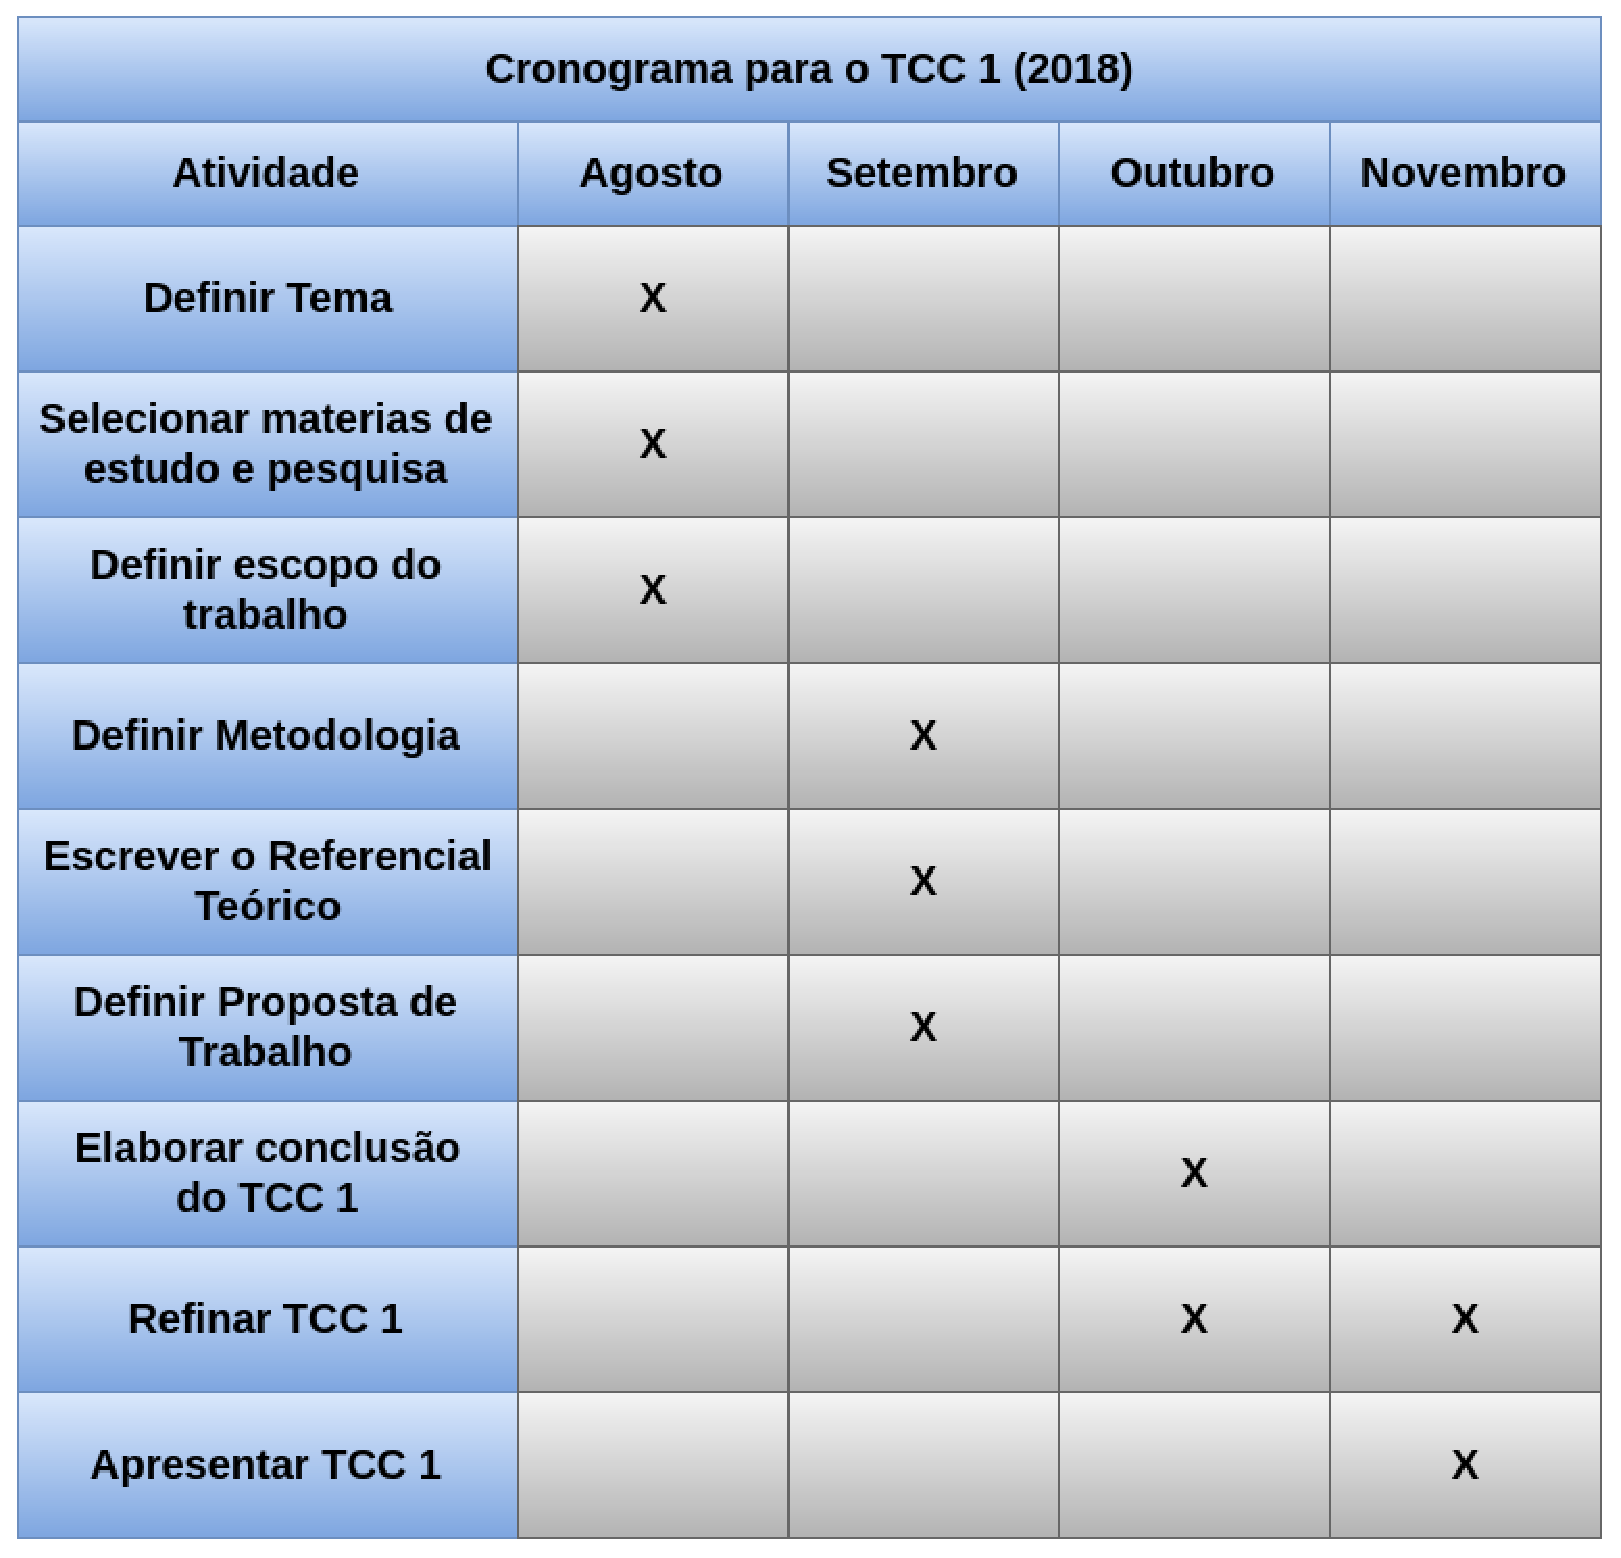
\includegraphics[keepaspectratio=true,scale=0.4]{figuras/cronograma_tcc1.eps}
  \caption[Cronograma do TCC 1.]{Cronograma do TCC 1. Fonte: Autor, baseado em \cite{leonardo}}
	\label{fig:cronograma_tcc1}
\end{figure}

\subsection{Marco 2: Trabalho de Conclusão de Curso 2}

A seguir são detalhados as atividades pertinentes do TCC 2:

\begin{itemize}
  \item \textbf{Efetuar ajustes propostos}:
  \begin{itemize}
    \item \textbf{Descrição}: Criar o documento do TCC 2 e efetuar ajustes do TCC 1 para o TCC 2
    \item \textbf{Entradas}: TCC 1
    \item \textbf{Saídas}: Corpo inicial do TCC 2.
  \end{itemize}
  \item \textbf{Documentar todos os resultados da metodologia aplicada}:
  \begin{itemize}
    \item \textbf{Descrição}: Documentar todos os artefatos definidos na metodologia de desenvolvimento.
    \item \textbf{Entradas}: Corpo inicial do TCC 2 e artefatos do software desenvolvidos.
    \item \textbf{Saídas}: Resultados do TCC 2.
  \end{itemize}
  \item \textbf{Documentar os resultados do Software}:
  \begin{itemize}
    \item \textbf{Descrição}: Documentar os resultados do produto final.
    \item \textbf{Entradas}: Software desenvolvido e Corpo inicial do TCC 2.
    \item \textbf{Saídas}: Resultados do TCC 2.
  \end{itemize}
  \item \textbf{Elaborar conclusão do TCC 2}:
  \begin{itemize}
    \item \textbf{Descrição}: Documentar a conclusão do TCC 2 e o que se pode esperar do software no futuro.
    \item \textbf{Entradas}: TCC 2
    \item \textbf{Saídas}: Conclusão do TCC 2.
  \end{itemize}
  \item \textbf{Refinar TCC 2}:
  \begin{itemize}
    \item \textbf{Descrição}: Fazer uma verificação geral no documento e melhorar alguns conteúdos, ortografia,
      gramática e outras erros encontrados.
    \item \textbf{Entradas}: TCC 2
    \item \textbf{Saídas}: TCC 2 refinado.
  \end{itemize}
  \item \textbf{Apresentar TCC 2}:
  \begin{itemize}
    \item \textbf{Descrição}: Criar slides e apresentar o TCC 2
    \item \textbf{Entradas}: TCC 2
    \item \textbf{Saídas}: Conclusão do trabalho.
  \end{itemize}
\end{itemize}

Em concordância com o processo de condução do TCC2 foi elaborado o seguinte cronograma:

\begin{figure}[h!]
	\centering
  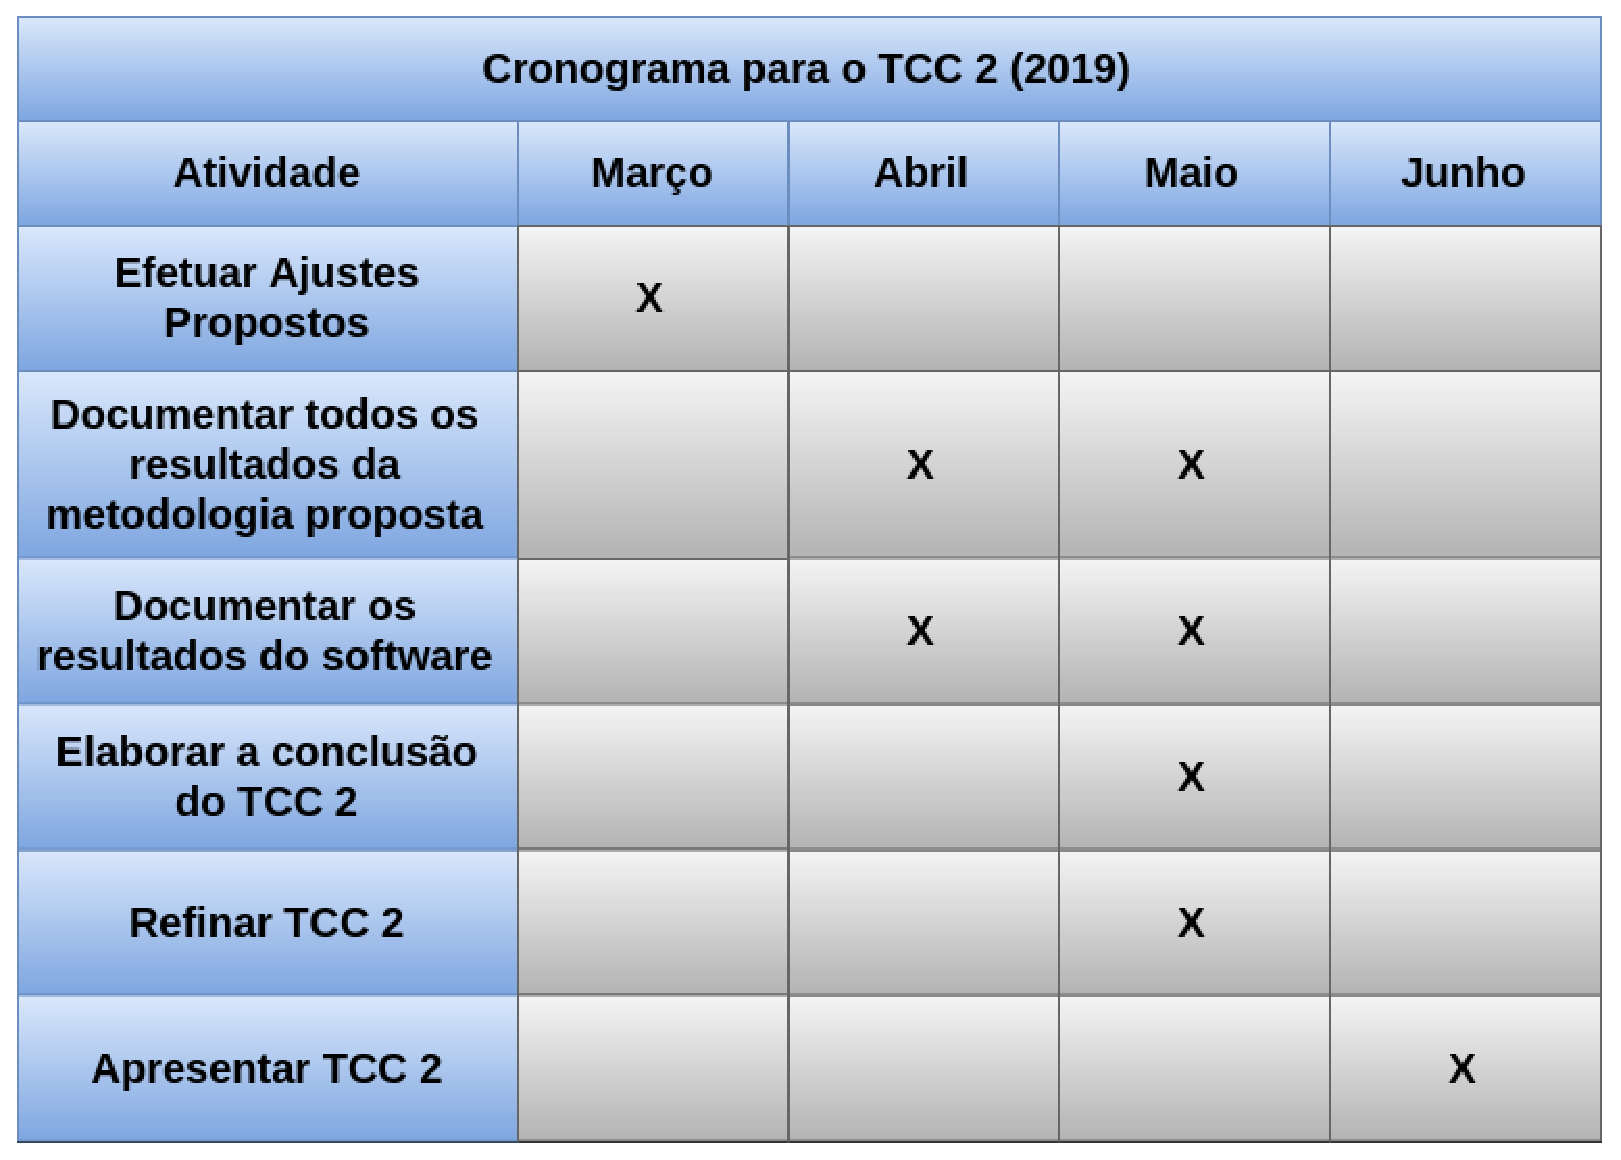
\includegraphics[keepaspectratio=true,scale=0.4]{figuras/cronograma_tcc2.eps}
  \caption[Cronograma do TCC 2.]{Cronograma do TCC 2. Fonte: Autor, baseado em \cite{leonardo}}
	\label{fig:cronograma_tcc2}
\end{figure}
